
\section{奇点的类型}

奇点往往用\trCompletion{}来定义最为简捷。

\textbf{28.2.1. \trhDefinition。}\quad 设 $X$ 是 $\bar{k}$ 上维数为 $1$ 的\trVariety，而 $p\in X$ 是一个\trClosedPoint。若 $\OO_{X,p}$ 在 $\mathfrak{m}_{X,p}$ 处的\trCompletion{}（作为拓扑环）\trIsomorphic{}于 $\bar{k}[[x,y]]/(xy)$，则称 $X$ 在 $p$ 处有一个\textbf{\trNode}。（这与 \S13.3.2 中\trNode{}的定义相比如何？）

\textbf{28.2.A.（练习）}\quad 设 $k=\bar{k}$ 且 $\operatorname{char}k\neq 2$。证明：$\mathbb{A}^2_k$ 中由 $y^2=x^2+x^3$ 截出的\trCurve{}在原点处有一个\trNode{}——自\cref{fig:normalization-nodal-cubic} 起，我们已经反复研究过这条曲线了。

\textbf{28.2.B.（练习）}\quad 设 $k=\bar{k}$，$\operatorname{char}k\neq 2$，并设有 $f(x,y)\in k[x,y]$。

(a)~证明：$\Spec k[x,y]/(f(x,y))$ 在原点处有一个\trNode，当且仅当 $f$ 没有次数为 $0$ 或 $1$ 的项，且其次数为 $2$ 的项不是一个完全平方。（这推广了\mbox{练习~28.2.A}。）

(b)~证明：$\Spec k[x,y]/(f(x,y))$ 在点 $(a,b)$ 处有一个\trNode，当且仅当
\[
\frac{\partial f}{\partial x}=\frac{\partial f}{\partial y}=0
\qquad\text{且}\qquad
\left(\frac{\partial^2 f}{\partial x^2}\right)\left(\frac{\partial^2 f}{\partial y^2}\right)\neq\left(\frac{\partial^2 f}{\partial x\,\partial y}\right)^{\!2}
\]
在 $(a,b)$ 处成立。

对于代数闭域上的\trVariety{}之外的情形，\trNode{}的定义要更成问题，我们给出几条可能的进路。对非代数闭域 $k$ 上的\trVariety，总可以\trBaseChange{}到代数闭包 $\bar{k}$。作为另一条进路，若 $p$ 是 $k$ 上（未必代数闭的）\trVariety{}的一个 $k$-\trValuedPoint，那么也可以径取同一个\mbox{定义~28.2.1}；如此得到的奇点可以合理地称作\emph{\trSplitNode}（split node），因为诸分支（或者更确切地说，诸切方向）是可分辨的。那些并\trNonSplitNode、但在\trBaseChange{}到 $\bar{k}$ 之后成为\trNode{}的奇点——诸如 $\Spec\mathbb{R}[x,y]/(x^2+y^2)$ 或 $\Spec\mathbb{Q}[x,y]/(x^2-2y^2)$ 的原点——可以合理地称作\emph{\trNonSplitNode}（non-split node）。

\textbf{28.2.2. \trhDefinition。}\quad 我们可以用类似的方式定义其他奇点。为免生枝节，我们在代数闭域上作定义。设 $X$ 是 $\bar{k}$ 上的\trVariety，$p$ 是 $X$ 的一个\trClosedPoint，其中 $\operatorname{char}k\neq 2$、$3$。若 $\hat{\OO}_{X,p}$ \trIsomorphic{}于 $\bar{k}[x,y]/(y^2-x^3)$ 的\trCompletion（相应地，$\bar{k}[x,y]/(y^2-x^4)$、$\bar{k}[x,y]/(y^3-x^3)$ 的\trCompletion），则称 $X$ 在 $p$ 处有一个\textbf{\trCusp}（相应地，\textbf{\trTacnode}、\textbf{\trTriplePoint{}}（triple point））。（前两种的图像见\cref{fig:plane-curve-singularities}。）若 $\hat{\OO}_{X,p}$ \trIsomorphic{}于 $\bar{k}[x,y]/(f(x,y))$ 的\trCompletion，其中 $f$ 是一个无重根的 $m$ 次\trHomogeneous{}多项式，则称 $X$ 在 $p$ 处有一个\textbf{重数 $m$ 的普通多重点}（ordinary multiple point of multiplicity $m$），或称\textbf{普通 $m$ 重点}（ordinary $m$-fold point）。（你可以很快看到：普通 $2$ 重点——或称\emph{普通二重点}（ordinary double point）——恰是一个\trNode，而普通 $3$ 重点是一个\trTriplePoint{}。）

\textbf{28.2.C.（平凡练习）}\quad （为简单起见，本练习在代数闭域上做。）定义 $A_n$ \textbf{曲线奇点}（curve singularity）（见 \S22.4.4）。定义 $A_n$ \textbf{曲面奇点}（surface singularity）（见\mbox{练习~22.4.F}）。定义 \textbf{$D_n$、$E_6$、$E_7$ 与 $E_8$ 曲面与曲线奇点}（surface and curve singularities）（见\mbox{注记~22.4.5}）。

\textbf{28.2.3. 使用这个定义。}\quad 现在我们给出一个例子，说明这个定义可以如何使用。

\textbf{28.2.D.（练习）}\quad 设 $X$ 是一个 $\bar{k}$-\trVariety，在\trClosedPoint{} $p$ 处有一个\trNode。证明：$X$ 在 $p$ 处的\trBlowup{}给出一个\trMorphism{} $\beta\colon\tilde{X}\to X$，其中\trExceptionalDivisor{} $\beta^{-1}(p)$ 由两个既约的光滑点组成。提示：利用「\trCompletion{}是\trFlat{}的」（\mbox{定理~28.1.6}(a)）与「胀开与平坦\trBaseChange{}交换」（\mbox{练习~24.1.P}(a)）这两个事实，把问题化归为对\trNode{}的「形式模型」$\Spec\bar{k}[x,y]/(xy)$ 的一个计算。

\textbf{28.2.E.（练习）}\quad 沿用上一个练习的术语，描述一个\trExactSequence
\begin{equation*}
\tag{28.2.3.1}\label{eq:node-blowup-ses}
0\longrightarrow\OO_X\longrightarrow\beta_*\OO_{\tilde{X}}\longrightarrow\OO_p\longrightarrow 0.
\end{equation*}
提示：\trFaithfullyFlat{}性。

\textbf{28.2.F.（练习）}\quad 我们沿用上两个练习的术语。设 $X$ 是纯维既约射影\trCurve，证明：$p_a(X)=p_a(\tilde{X})+1$。

于是，「解消一个\trNode」使\trCurve{}的\trArithmeticGenus{}减少 $1$。如果你愿意，你不难进一步证明：「解消一个\trCusp」使亏格减少 $1$，而「解消一个\trTacnode」使亏格减少 $2$。一般地，对每一类\trCurve\trSingularPoint，它对亏格的贡献——也就是（当\trCurve{}是射影时）这条\trCurve{}的亏格与其「在该\trSingularPoint{}处的部分\trNormalization」的亏格之差——称为\textbf{\trDeltaInvariant}（$\delta$-invariant）。于是，\trNode{}或\trCusp{}的 $\delta$ 为 $1$，而\trTacnode{}的 $\delta$ 为 $2$。

\textbf{28.2.G.（练习）}\quad 证明：对\emph{任何}奇点类型（除光滑点以外），都有 $\delta>0$。

\textbf{28.2.H.（练习）}\quad 证明：既约不可约的 $d$ 次平面\trCurve{}至多能有 $\binom{d-1}{2}$ 个\trSingularPoint。

\textbf{28.2.I.（练习）}\quad 有一个非正式的小窍门，可以在结点（射影既约）\trCurve{}于例子中出现时迅速算出其亏格。在画得出来的前提下，在一张纸上（也就是实平面）画一幅草图，使\trNode{}「看上去像\trNode」，并且亏格为 $g$ 的\trCurve{}被画有 $g$ 个洞，如\cref{fig:genus-count-sketch} 那样。（在\cref{fig:genus-count-sketch} 中，我们看到四个\trIrreducibleComponent，其\trGeometricGenus{}分别为 $0$、$0$、$1$ 与 $3$；前三个分量是光滑的，而第四个与自身相交一次；此外还有六个\trNode。）然后，若这条\trCurve{}\trConnected，就数一数图中看得见的洞的个数。证明这套口诀确实有效。（若\trCurve{}不连通时该怎么办，也请自行琢磨。）

\begin{figure}[htbp]
\centering
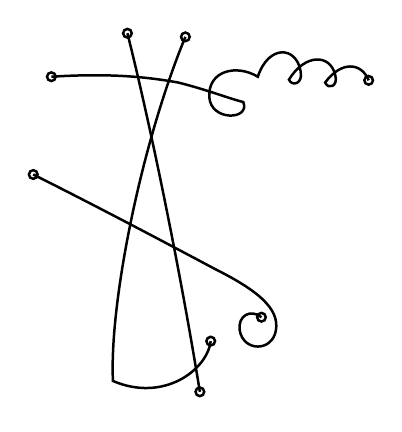
\begin{tikzpicture}[line width=0.9pt, scale=0.92]
  \draw (2.15,2.45) .. controls (1.55,1.00) and (1.10,-1.20) .. (1.15,-2.30)
        .. controls (1.85,-2.60) and (2.45,-2.15) .. (2.50,-1.75);
  \draw (1.35,2.50) .. controls (1.70,1.10) and (2.10,-0.90) .. (2.35,-2.45);
  \draw (0.05,0.55) .. controls (0.85,0.15) and (1.80,-0.35) .. (2.55,-0.75)
        .. controls (3.15,-1.05) and (3.45,-1.30) .. (3.40,-1.60)
        .. controls (3.35,-1.90) and (2.95,-1.90) .. (2.90,-1.60)
        .. controls (2.87,-1.40) and (3.05,-1.30) .. (3.20,-1.42);
  \draw (0.30,1.90) .. controls (1.10,1.95) and (1.60,1.90) .. (2.05,1.82)
        .. controls (2.45,1.72) and (2.75,1.60) .. (2.95,1.55)
        .. controls (3.05,1.30) and (2.50,1.28) .. (2.48,1.62)
        .. controls (2.46,1.98) and (2.85,2.08) .. (3.15,1.90)
        .. controls (3.30,2.35) and (3.68,2.32) .. (3.74,1.98)
        .. controls (3.78,1.80) and (3.62,1.76) .. (3.58,1.86)
        .. controls (3.80,2.22) and (4.15,2.22) .. (4.22,1.92)
        .. controls (4.26,1.76) and (4.12,1.72) .. (4.08,1.82)
        .. controls (4.30,2.12) and (4.58,2.10) .. (4.68,1.85);
  \draw (2.15,2.45) circle (1.7pt);
  \draw (2.50,-1.75) circle (1.7pt);
  \draw (1.35,2.50) circle (1.7pt);
  \draw (2.35,-2.45) circle (1.7pt);
  \draw (0.05,0.55) circle (1.7pt);
  \draw (3.20,-1.42) circle (1.7pt);
  \draw (0.30,1.90) circle (1.7pt);
  \draw (4.68,1.85) circle (1.7pt);
\end{tikzpicture}
\caption{这条\trCurve{}的亏格为 $8$（数一数那些「洞」！）。（依原书手绘图重绘。）}\label{fig:genus-count-sketch}
\end{figure}

\textbf{28.2.4.}\quad 这可能相当有用。例如，\cref{fig:arith-genus-sketches} 中的几幅草图可以提醒你：$d$ 次平面\trCurve{}的\trArithmeticGenus{}为 $\binom{d-1}{2}$；$\mathbb{P}^1\times\mathbb{P}^1$ 上由 $\OO(a,b)$ 的一个\trSection{}给出的\trCurve{}具有亏格 $(a-1)(b-1)$（\S15.2.10）；而 \trHirzebruchSurface{} $\mathbb{F}_2$ 上类为 $2C+2F$ 的\trCurve{}（使用\mbox{练习~20.2.M} 的语言）的\trArithmeticGenus{}为 $3$。在每一种情形，我们都是在该类中取一条合适的\trCurve，利用「\trArithmeticGenus{}在\trFlat\trFamily{}中是常数」这一事实（\mbox{关键练习~24.7.A}）。

\begin{figure}[htbp]
\centering
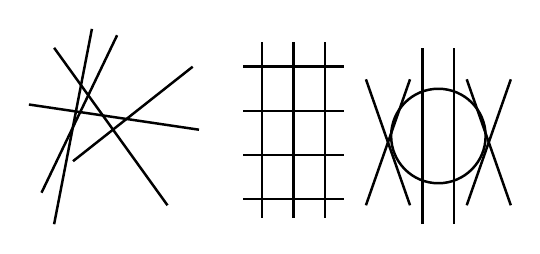
\begin{tikzpicture}[line width=0.9pt, scale=0.8]
  \draw (-0.10,2.40) -- (1.70,-0.10);
  \draw (0.90,2.60) -- (-0.30,0.10);
  \draw (-0.50,1.50) -- (2.20,1.10);
  \draw (0.20,0.60) -- (2.10,2.10);
  \draw (0.50,2.70) -- (-0.10,-0.40);
  \draw (3.20,-0.30) -- (3.20,2.50);
  \draw (3.70,-0.30) -- (3.70,2.50);
  \draw (4.20,-0.30) -- (4.20,2.50);
  \draw (2.90,0.00) -- (4.50,0.00);
  \draw (2.90,0.70) -- (4.50,0.70);
  \draw (2.90,1.40) -- (4.50,1.40);
  \draw (2.90,2.10) -- (4.50,2.10);
  \draw (6.00,1.00) circle (0.75);
  \draw (5.75,-0.40) -- (5.75,2.40);
  \draw (6.25,-0.40) -- (6.25,2.40);
  \draw (4.85,1.90) -- (5.55,-0.10);
  \draw (4.85,-0.10) -- (5.55,1.90);
  \draw (6.45,1.90) -- (7.15,-0.10);
  \draw (6.45,-0.10) -- (7.15,1.90);
\end{tikzpicture}
\caption{这三条\trCurve{}的\trArithmeticGenus{}分别为 $6$、$6$ 与 $3$。（依原书手绘图重绘。）}\label{fig:arith-genus-sketches}
\end{figure}

\textbf{28.2.5. 其他定义。}\quad 若 $\bar{k}=\mathbb{C}$，则这一类定义与解析定义相吻合（见 [Ar1, \S1]）。例如，一个复代数\trCurve\trSingularPoint{}是\trNode，当且仅当它\trAnalyticallyIsomorphic{}于 $\mathbb{C}^2$ 中 $xy=0$ 的一个开邻域。还有一种「平展局部」的\trIsomorphism{}概念，我们在此不作定义。同样地，这也导致这几类奇点的同一个定义（见 [Ar2, \S2]）。
